\documentclass[a4paper, 12pt]{article}
\linespread{1.15} %interlinea
\pagestyle{plain}
\usepackage{geometry} %margini
\usepackage[]{tabto}
\geometry{a4paper, top=3cm, bottom=3cm, left=3cm, right=3cm, bindingoffset=5mm}
\usepackage{graphicx}
\usepackage{adjustbox}
\graphicspath{Documentazione/Immagini/}
\usepackage{multicol} %più colonne
\usepackage{ragged2e} %allineamento testo
\usepackage{float}
\usepackage{inconsolata}
\usepackage[]{fancyhdr}
\usepackage[utf8]{inputenc}
\usepackage{array}
\usepackage{tabularx}
\usepackage{geometry}
\usepackage{enumitem}
\usepackage{multirow}
\usepackage{longtable}
\usepackage{tcolorbox}
\tcbuselibrary{skins}

\geometry{margin=2.3cm}
\renewcommand{\arraystretch}{1.2} % Aumenta altezza delle righe
\setlist[itemize]{left=0pt, label=\textbullet, itemsep=1pt, topsep=1pt}
\definecolor{linecolor}{RGB}{200, 200, 200}

\newtcolorbox{graybox}{
	colback=gray!15,
	colframe=gray!15,
	boxrule=0pt,
	left=1em,
	top=4pt,          % Spazio interno superiore
	bottom=4pt,       % Spazio interno inferiore
	before skip=4pt,  % Spazio prima del box
	after skip=6pt,   % Rimuove spazio aggiuntivo automatico
	enhanced,
	sharp corners
}

\pagestyle{fancy}
\fancyhead{}
\cfoot{\thepage}
\lfoot{Gioele Manzoni}
\rfoot{Luca Lucci}
\author{Gioele Manzoni}
\title{Documentazione per Progettazione Base di Dati}
\begin{document}
	\begin{center}
		\begin{figure}[hb]
			
\includegraphics[width=1\textwidth]{../Immagini/coverpic.png}
		\end{figure}
		{\LARGE DOCUMENTAZIONE PER PROGETTAZIONE \\BASE DI DATI \par}
		{\Large{Progetto in Carico: Hackathon \par}}
		\vfill
		{\large{\textbf{\textsc{CdL Triennale in Informatica}}}}\\
		{\large{\textsc{Corso di Basi di Dati I}}}\\
		{\large{\textsc{GIOELE MANZONI}}}\\
		{\large{\textsc{N86004562}}}\\
		{\large{\textsc{LUCA LUCCI}}}\\
		{\large{\textsc{N86005180}}}\\
		{\large{\textsc{\today}}}\\
		\Large{\textsc{Anno Accademico: 2024/2025}}
	\end{center}
	\newpage
	\tableofcontents
	\newpage
	\section{Introduzione}
	Questa documentazione descriverà il processo di progettazione e sviluppo di un Database relazionale che gestirà il flusso di dati di un applicativo dedicato all'organizzazione di Hackathon. Questo è un progetto a cura degli studenti Gioele Manzoni e Luca Lucci del CdL di Informatica presso l'Università degli Studi di Napoli "Federico II".
	\subsection{Traccia del Progetto}
	Un hackathon, ovvero una "maratona di hacking", è un evento durante il quale team di partecipanti si sfidano per progettare e implementare nuove soluzioni basate su una certa tecnologia o mirate a un certo ambito applicativo. 
	Ogni hackathon ha un titolo identificativo, si svolge in una certa sede e in un certo intervallo di tempo (solitamente 2 giorni) e ha un organizzatore specifico (registrato alla piattaforma). L'organizzatore seleziona un gruppo di giudici (selezionati tra gli utenti della piattaforma, invitandoli). Infine, l'organizzatore apre le registrazioni, che si chiuderanno 2 giorni prima dell'evento. Ogni evento avrà un numero massimo di iscritti e una dimensione massima del team.
	Durante il periodo di registrazione, gli utenti possono registrarsi per l'Hackathon di loro scelta (eventualmente registrandosi sulla piattaforma se non lo hanno già fatto). Una volta iscritti, gli utenti possono formare team. I team diventano definitivi quando si chiudono le iscrizioni. All'inizio dell'hackathon, i giudici pubblicano una descrizione del problema da affrontare. 
	Durante l'hackathon, i team lavorano separatamente per risolvere il problema e devono caricare periodicamente gli aggiornamenti sui "progressi" sulla piattaforma come documento, che può essere esaminato e commentato dai giudici. Alla fine dell'hackathon, ogni giudice assegna un voto (da 0 a 10) a ciascun team e la piattaforma, dopo aver acquisito tutti i voti, pubblica le classifiche dei team.
	
	
	\subsection*{Caratteristiche dell'Hackathon}
	
	Ogni Hackathon ha le seguenti caratteristiche:
	
	\begin{itemize}
		\item Un \textbf{titolo identificativo};
		\item Una \textbf{sede} in cui si svolge;
		\item Un \textbf{intervallo di tempo}, solitamente di due giorni;
		\item Un \textbf{organizzatore specifico}, registrato sulla piattaforma.
	\end{itemize}
	
	\subsection*{Giudici e Registrazioni}
	
	\begin{itemize}
		\item L'organizzatore seleziona un gruppo di \textbf{giudici}, invitandoli tra gli utenti registrati sulla piattaforma.
		\item L'organizzatore apre le \textbf{registrazioni}, che si chiudono due giorni prima dell'inizio dell'evento.
		\item Ogni evento prevede un \textbf{numero massimo di iscritti} e una \textbf{dimensione massima del team}.
		\item Durante il periodo di registrazione, gli utenti possono registrarsi all'Hackathon di loro scelta, previa registrazione sulla piattaforma se non ancora effettuata.
	\end{itemize}
	
	\subsection*{Formazione dei Team}
	
	\begin{itemize}
		\item Una volta iscritti, gli utenti possono \textbf{formare team}.
		\item I team diventano \textbf{definitivi alla chiusura delle iscrizioni}.
	\end{itemize}
	
	\subsection*{Svolgimento dell'Hackathon}
	
	\begin{itemize}
		\item All'inizio dell'evento, i giudici \textbf{pubblicano una descrizione del problema} da affrontare.
		\item Durante l’Hackathon, i team lavorano separatamente per risolvere il problema.
		\item I team devono \textbf{caricare periodicamente aggiornamenti sui progressi} tramite documenti sulla piattaforma.
		\item I documenti possono essere \textbf{esaminati e commentati dai giudici}.
	\end{itemize}
	
	\subsection*{Valutazione e Classifica}
	
	\begin{itemize}
		\item Alla fine dell'Hackathon, ogni giudice assegna un \textbf{voto da 0 a 10} a ciascun team.
		\item La piattaforma, dopo aver acquisito tutti i voti, \textbf{pubblica le classifiche dei team}.
	\end{itemize}
	
	\newpage
	\section{Progettazione Concettuale}
	\begin{figure}[H]
		\centering
		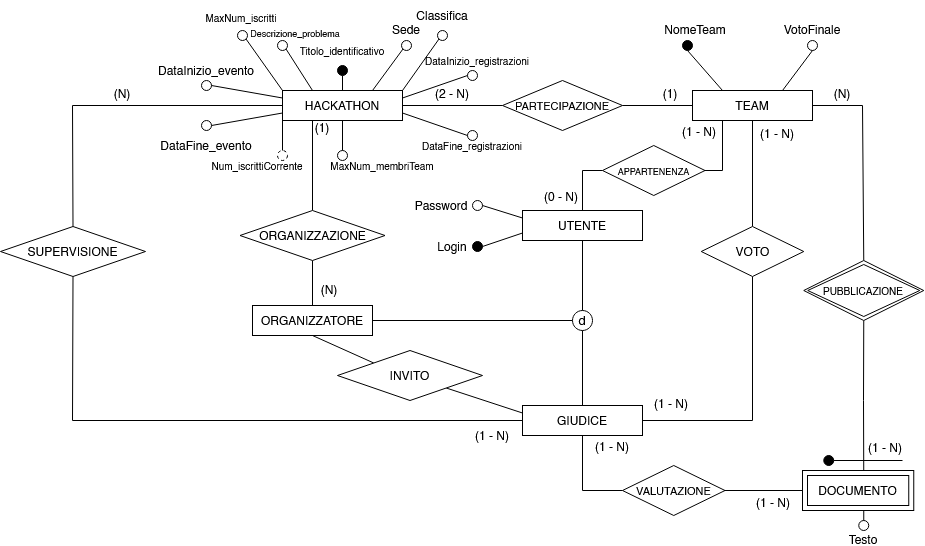
\includegraphics[width=1\textwidth]{../Immagini/EERDiagram_Hackathon}
		\caption[Grafico UML]{Grafico UML Concettuale}
	\end{figure}
	\subsection{Analisi delle Entità e degli Attributi}
	Seguendo la traccia, nella fase di progettazione concettuale sono state trovate le suddette entità:
	\subsubsection{Hackathon}
	Entità dedicata a tutte le maratone di Hacking organizzate.
	\begin{itemize}
		\item \textbf{Hackathon} ($\underline{Titolo\_identificativo}$, Descrizione\_problema, Sede, Classifica,\\ DataInizio\_registrazioni, DataFine\_registrazioni, DataInizio\_Evento, DataFine\_Evento, \\Num\_iscrittiCorrente, MaxNum\_membriTeam, MaxNum\_iscritti)
	\end{itemize}
	\subsubsection{Utente}
	Generalizzazione dedicata a tutti i tipi di utenti che è possibile avere all'interno della piattaforma.
	La generalizzazione è considerata come \textbf{DISGIUNTA PARZIALE}, poiché è possibile avere utenti della piattaforma che non sono né organizzatori né giudici.
	\begin{itemize}
		\item \textbf{Utente} ($\underline{Login}$, Password)
	\end{itemize}
	\subsubsection{Organizzatore}
	Specializzazione dell'entità \textbf{Utente}, rappresentante gli organizzatori di maratone di Hacking.
	Non possiede alcun attributo specifico a sé stesso, la sua specializzazione definisce soltanto gli utenti con le giuste credenziali per poter gestire la piattaforma.
	\subsubsection{Giudice}
	Specializzazione dell'entità \textbf{Utente}, rappresentante i giudici che daranno le loro valutazioni ai documenti e supervisioneranno le Hackathon.
	\subsubsection{Team}
	Entità che definisce una squadra organizzata da un Utente e composta da N Utenti.
	\begin{itemize}
		\item \textbf{Conferenza} ($\underline{NomeTeam}$, VotoFinale)
	\end{itemize}
	\subsubsection{Documento}
	Entità debole che definisce un documento scritto da un team.
	\begin{itemize}
		\item \textbf{Documento} ($\underline{NomeTeam}$, Testo)
	\end{itemize}
	\subsection{Analisi delle Relazioni}
	Qui verranno descritte tutte le relazioni e le specializzazioni presenti all'interno della struttura concettuale non ancora ristrutturata.
	\begin{itemize}
		\item \textit{Organizzazione} (\textbf{Hackathon} - \textbf{Organizzatore}: 1 - N):\\Un Hackathon può essere organizzata da un solo organizzatore. Un organizzatore può organizzare più Hackathon.
		\item \textit{Partecipazione} (\textbf{Team} - \textbf{Hackathon}: 1 - 2..N):\\Un Team può partecipare ad una sola Hackathon. Un Hackathon, per essere valida, deve avere un minimo di 2 Team fino ad un massimo di N.
		\item \textit{Supervisione} (\textbf{Giudice} - \textbf{Hackathon}: 1..N - N):\\Un Giudice può supervisionare N Hackathon. Un Hackathon deve essere monitorata da almeno un giudice.
		\item \textit{Appartenenza} (\textbf{Utente} - \textbf{Team}: 0..N - 1..N):\\Un Utente può partecipare ad uno o più team, o può non parteciparci affatto. Un Team deve essere composto da un minimo di un Utente fino ad un massimo di N (il limite di utenti appartenenti ad un Team è deciso dall'Hackathon alla quale si partecipa).
		\item \textit{Invito} (\textbf{Giudice} - \textbf{Hackathon}: 1..N - 1..N):\\Un giudice deve invitare un minimo di un utente fino ad un massimo di N utenti per essere giudici. Un giudice, per ricevere un invito, deve riceverlo da almeno un organizzatore.
		\item \textit{Voto} (\textbf{Giudice} - \textbf{Team}: 1..N - 1..N):\\Un Giudice può esprimere una votazione ad un minimo di un Team. Un team può ricevere voti da almeno un giudice.
		\item \textit{Valutazione} (\textbf{Giudice} - \textbf{Documento}: 1..N - 1..N):\\Un Giudice deve esprimere una valutazione per almeno un documento. Un documento deve ottenere una valutazione da almeno un giudice.
		\item \textit{Pubblicazione} (\textbf{Documento} - \textbf{Team}: 1..N - N):\\Relazione identificante per l'entità debole Documento, in quanto generato direttamente da un Team e non può esistere senza un associazione ad un Team.
	\end{itemize}
	\newpage
	\subsection{Ristrutturazione del Modello Concettuale}
	Dopo aver analizzato i requisiti, le entità e le relazioni ed aver prodotto uno schema concettuale passeremo alla sua Ristrutturazione, seguendo i passaggi necessari elencati nelle prossime sottosezioni, ordinate in:
	\begin{itemize}
		\item Analisi delle Ridondanze
		\item Analisi delle Generalizzazioni/Gerarchie di Specializzazione
		\item Analisi degli Attributi Multivalore
		\item Analisi degli Attributi Strutturati
		\item Partizionamento/Accorpamento di Entità e Relazioni
		\item Analisi delle Chiavi
	\end{itemize}
	\subsubsection{Analisi delle Ridondanze}
	\subsubsection{Analisi delle Generalizzazioni/Gerarchie di Specializzazione}
	\subsubsection{Analisi degli Attributi Multivalore}
	\subsubsection{Analisi degli Attributi Strutturati}
	\subsubsection{Partizionamento/Accorpamento di Entità e Relazioni}
	\subsubsection{Analisi delle Chiavi}
	\subsection{Class Diagram Ristrutturato}
	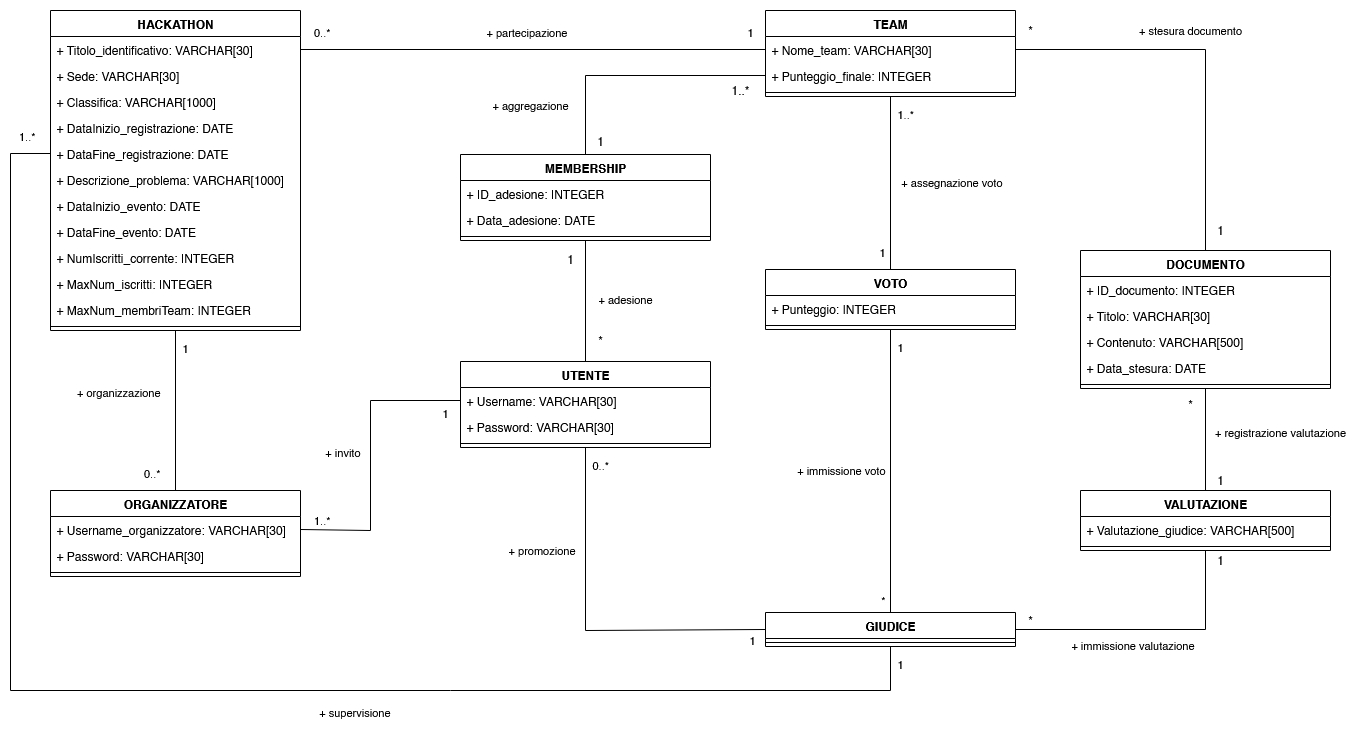
\includegraphics[width=1\textwidth]{../Immagini/Hackathon_UMLRistrutturato}
	\newpage
	\subsection{Dizionario delle Classi}
	{\footnotesize % Testo più piccolo ma leggibile
		\setlength{\arrayrulewidth}{0.5pt}  % Opzionale: regola lo spessore
		\renewcommand{\arraystretch}{1.2}  % Opzionale: aumenta lo spazio tra le righe
		\begin{longtable}{
			>{\raggedright\arraybackslash}p{4cm} % Colonna 1: allineamento a sinistra
			>{\centering\arraybackslash}p{4cm}    % Colonna 2: centrato
			>{\raggedright\arraybackslash}p{6.5cm}% Colonna 3: allineamento a sinistra
			}
			\hline
			\textbf{Classe} & \textbf{Descrizione} & \textbf{Attributi} \\
			\hline
			\endfirsthead
			\hline
			\textbf{Classe} & \textbf{Descrizione} & \textbf{Attributi} \\
			\hline
			\endhead
			\hline
			\endfoot
			\hline
			\endlastfoot
			
			\textbf{HACKATHON} &
			Evento organizzato a cui partecipano team. &
			\begin{itemize}
				\item \texttt{Titolo\_identificativo} (VARCHAR[30]): Titolo univoco che identifica un Hackathon;
				\item \texttt{Sede} (VARCHAR[30]): Sede dove si svolgerà l'Hackathon;
				\item \texttt{Classifica} (VARCHAR[1000]): Classifica finale con i posizionamenti dei Team, in ordine di punteggio complessivo;
				\item \texttt{DataInizio\_registrazione} (DATE);
				\item \texttt{DataFine\_registrazione} (DATE);
				\item \texttt{Descrizione\_problema} (VARCHAR[1000]): Descrizione del problema da risolvere offerta dai giudici;
				\item \texttt{DataInizio\_evento} (DATE);
				\item \texttt{DataFine\_evento} (DATE);
				\item \texttt{NumIscritti\_corrente} (INTEGER): Numero degli iscritti all'Hackathon aggiornato fino alla chiusura delle iscrizioni o al raggiungimento del tetto massimo;
				\item \texttt{MaxNum\_iscritti} (INTEGER): Numero massimo di iscritti per un Hackathon;
				\item \texttt{MaxNum\_membriTeam} (INTEGER): Numero massimo di membri per team iscritti ad una determinata Hackathon;
			\end{itemize} \\
			\hline
			
			\textbf{UTENTE} &
			Utente registrato nel sistema. &
			\begin{itemize}
				\item \texttt{Username} (VARCHAR[30]): Nome utente univoco;
				\item \texttt{Password} (VARCHAR[30])
			\end{itemize} \\
			\hline
			
			\textbf{ORGANIZZATORE} &
			Utente con ruolo di organizzatore. &
			\begin{itemize}
				\item \texttt{Username\_organizzatore} (VARCHAR[30]): Nome utente univoco per organizzatore;
				\item \texttt{Password} (VARCHAR[30])
			\end{itemize} \\
			\hline
			
			\textbf{GIUDICE} &
			Utente con ruolo di giudice. &
			\begin{itemize}
				\item \texttt{ID\_giudice} (INTEGER): Codice identificativo che ordina ciascun giudice alla propria Hackathon in ordine di adesione;
			\end{itemize} \\
			\hline
			
			\textbf{TEAM} &
			Team partecipante a un hackathon. &
			\begin{itemize}
				\item \texttt{Nome\_team} (VARCHAR[30]): Nome univoco che identifica un team;
				\item \texttt{Punteggio\_finale} (INTEGER): Punteggio complessivo del team dato dalla somma di tutti i punteggi ottenuti dai giudici;
			\end{itemize} \\
			\hline
			
			\textbf{MEMBERSHIP} &
			Adesione di un utente a un team. &
			\begin{itemize}
				\item \texttt{ID\_adesione} (INTEGER): Codice identificativo per la singola adesione ad un Team;
				\item \texttt{Data\_adesione} (DATE)
			\end{itemize} \\
			\hline
			
			\textbf{VOTO} &
			Voto assegnato da un giudice a un team. &
			\begin{itemize}
				\item \texttt{Punteggio} (INTEGER)
			\end{itemize} \\
			\hline
			
			\textbf{DOCUMENTO} &
			Documento prodotto da un team. &
			\begin{itemize}
				\item \texttt{ID\_documento} (INTEGER): Codice identificativo per il singolo documento;
				\item \texttt{Titolo} (VARCHAR[30]): Titolo del documento per riassumerne il contenuto;
				\item \texttt{Contenuto} (VARCHAR[500]): Testo del documento;
				\item \texttt{Data\_stesura} (DATE)
			\end{itemize} \\
			\hline
			
			\textbf{VALUTAZIONE} &
			Valutazione scritta da un giudice. &
			\begin{itemize}
				\item \texttt{Valutazione\_giudice} (VARCHAR[500]): Valutazione di un giudice per un documento;
			\end{itemize} \\
			\hline
			
		\end{longtable}
	}
	\newpage
	\subsection{Dizionario delle Associazioni}
	{\footnotesize
		\setlength{\arrayrulewidth}{0.5pt}
		\renewcommand{\arraystretch}{1.5}
		\begin{longtable}{
				>{\raggedright\arraybackslash}p{4cm} % Colonna 1: allineamento a sinistra
				>{\centering\arraybackslash}p{4cm}    % Colonna 2: centrato
				>{\raggedright\arraybackslash}p{6.5cm}% Colonna 3: allineamento a sinistra
			}
			\hline
			\textbf{Nome Associazione} & \textbf{Entità Associate} & \textbf{Descrizione Associazione} \\
			\hline
			\endfirsthead
			\hline
			\textbf{Nome Associazione} & \textbf{Entità Associate} & \textbf{Descrizione Associazione} \\
			\hline
			\endhead
			\hline
			\endfoot
			\hline
			\endlastfoot
			
			\textbf{Partecipazione}  & 
			HACKATHON $\leftrightarrow$ TEAM &
			\begin{itemize}
				\item Tipo: Uno-a-molti [0..1 - *]
				\item Un Hackathon può avere più Team partecipanti. Un Team deve partecipare ad un Hackathon
				\item Chiave esterna: \texttt{Titolo\_hackathon} in TEAM
				\item Vincolo: Ogni Team partecipa a un solo Hackathon
			\end{itemize} \\
			\hline
			
			\textbf{Organizzazione} & 
			ORGANIZZATORE $\leftrightarrow$ HACKATHON &
			\begin{itemize}
				\item Tipo: Uno-a-molti [0..* - 1]
				\item Un organizzatore può organizzare più Hackathon, o può non organizzarne. Un Hackathon è organizzata da un solo organizzatore
				\item Chiave esterna: \texttt{Username\_organizzatore} in ORGANIZZATORE
				\item Vincolo: Ciascun Hackathon può essere organizzata da una sola persona
			\end{itemize} \\
			\hline
			
			\textbf{Supervisione} & 
			HACKATHON $\leftrightarrow$ GIUDICE &
			\begin{itemize}
				\item Tipo: Uno-a-molti [1..* - 1]
				\item Un Hackathon può avere più Giudici assegnati
				\item Chiave esterna: \texttt{Titolo\_hackathon} in GIUDICE
				\item Vincolo: Ogni Giudice è assegnato a un solo Hackathon
			\end{itemize} \\
			\hline
			
			\textbf{Invito} & 
			ORGANIZZATORE $\leftrightarrow$ UTENTE &
			\begin{itemize}
				\item Tipo: Uno-a-molti [1..* - 1]
				\item Un organizzatore deve invitare almeno un utente a diventare giudice
				\item Vincolo: Un utente può ricevere un solo invito alla volta per essere giudice di un Hackathon
			\end{itemize} \\
			\hline
			
			\textbf{Aggregazione} & 
			TEAM $\leftrightarrow$ MEMBERSHIP &
			\begin{itemize}
				\item Tipo: Uno-a-molti [1..* - 1]
				\item Un Team può avere più adesioni (Membership)
				\item Chiave esterna: \texttt{Nome\_team} in MEMBERSHIP
				\item Vincolo: Ogni Membership è per un solo Team
			\end{itemize} \\
			\hline
			
			\textbf{Adesione} & 
			UTENTE $\leftrightarrow$ MEMBERSHIP &
			\begin{itemize}
				\item Tipo: Uno-a-molti [* - 1]
				\item Un Utente può appartenere a più Team (tramite Membership)
				\item Chiave esterna: \texttt{Username\_utente} in MEMBERSHIP
				\item Vincolo: Ogni Membership è di un solo Utente ed è rivolta ad un solo Team
			\end{itemize} \\
			\hline
			
			\textbf{Stesura Documento} & 
			TEAM $\leftrightarrow$ DOCUMENTO &
			\begin{itemize}
				\item Tipo: Uno-a-molti [* - 1]
				\item Un Team può produrre più Documenti
				\item Chiavi esterne: \texttt{Nome\_team} e \texttt{Titolo\_hackathon} in DOCUMENTO
				\item Vincolo: Ogni Documento è prodotto da un solo Team
			\end{itemize} \\
			\hline
			
			\textbf{Registrazione Valutazione} & 
			DOCUMENTO $\leftrightarrow$ VALUTAZIONE &
			\begin{itemize}
				\item Tipo: Uno-a-molti [* - 1]
				\item Un Documento può ricevere più Valutazioni
				\item Chiave esterna: \texttt{ID\_documento} in VALUTAZIONE
				\item Vincolo: Ogni Valutazione è per un solo Documento
			\end{itemize} \\
			\hline
			
			\textbf{Immissione Valutazione} & 
			GIUDICE $\leftrightarrow$ VALUTAZIONE &
			\begin{itemize}
				\item Tipo: Uno-a-molti [* - 1]
				\item Un Giudice può scrivere più Valutazioni
				\item Chiavi esterne: \texttt{ID\_giudice} e \texttt{Username\_giudice} in VALUTAZIONE
				\item Vincolo: Ogni Valutazione è scritta da un solo Giudice
			\end{itemize} \\
			\hline
			
			\textbf{Immissione Voto} & 
			GIUDICE $\leftrightarrow$ VOTO &
			\begin{itemize}
				\item Tipo: Uno-a-molti [* - 1]
				\item Un Giudice può assegnare più Voti
				\item Chiavi esterne: \texttt{ID\_giudice} e \texttt{Username\_giudice} in VOTO
				\item Vincolo: Ogni Voto è assegnato da un solo Giudice
			\end{itemize} \\
			\hline
			
			\textbf{Assegnazione Voto} & 
			TEAM $\leftrightarrow$ VOTO &
			\begin{itemize}
				\item Tipo: Uno-a-molti [1..* - 1]
				\item Un Team può ricevere più Voti
				\item Chiavi esterne: \texttt{Nome\_team} e \texttt{Titolo\_hackathon} in VOTO
				\item Vincolo: Ogni Voto è assegnato a un solo Team
			\end{itemize} \\
			\hline
		\end{longtable}
	}
	\newpage
	\subsection{Dizionario dei Vincoli}
	{\footnotesize
		\setlength{\arrayrulewidth}{0.5pt}
		\renewcommand{\arraystretch}{1.5}
		\begin{longtable}{
				>{\raggedright\arraybackslash}p{5.5cm}
				>{\raggedright\arraybackslash}p{10cm}
			}
			\hline
			\textbf{Nome Vincolo} & \textbf{Descrizione} \\
			\hline
			\endfirsthead
			\hline
			\textbf{Nome Vincolo} & \textbf{Descrizione} \\
			\hline
			\endhead
			\hline
			\endfoot
			\hline
			\endlastfoot
			
			\textbf{Chiusura Registrazioni} &
			Le registrazioni devono chiudersi 2 giorni prima dell'evento:
			\texttt{DataFine\_registrazione} = \texttt{DataInizio\_evento} - 2 giorni \\
			\hline
			
			\textbf{Range Voti} &
			I voti assegnati dai giudici devono essere interi compresi tra 0 e 10\\
			\hline
			
			\textbf{Numero Minimo Membri Team} &
			Ogni team deve avere almeno 2 membri per essere valido \\
			\hline
			
			\textbf{Numero Massimo Membri Team} &
			Un team non può superare il numero massimo di membri definito nell'Hackathon \\
			\hline
			
			\textbf{Documentazione Obbligatoria} &
			Ogni team deve aver caricato almeno un documento per essere valutato \\
			\hline
			
			\textbf{Temporalità Documenti} &
			I documenti possono essere caricati solo durante l'Hackathon\\
			\hline
			
			\textbf{Unicità Voto Giudice} &
			Un giudice non può votare più volte lo stesso team\\
			\hline
			
			\textbf{Classifica Automatica} &
			La classifica deve essere generata automaticamente come media dei voti\\
			\hline
			
			\textbf{Singolo Ruolo} &
			Un utente non può essere contemporaneamente organizzatore e giudice nello stesso Hackathon \\
			\hline
			
			\textbf{Completezza Valutazioni} &
			Tutti i giudici devono aver votato prima della pubblicazione della classifica \\
			\hline
			
			\textbf{Blocco Team} &
			I team non possono essere modificati dopo la chiusura delle registrazioni
		\end{longtable}
	}
	\newpage
	\section{Progettazione Logica}
	\subsection{Schema Logico}
	\begin{itemize}
		\item \texttt{Hackathon(\underline{Titolo\_identificativo}, \underline{\underline{Username\_organizzatore}}, Sede, Classifica,\\
			DataInizio\_registrazione, DataFine\_registrazione, Descrizione\_problema, 
			\\DataInizio\_evento, DataFine\_evento, NumIscritti\_corrente, MaxNum\_iscritti, MaxNum\_membriTeam)}
		\begin{graybox}
			\texttt{Username\_organizzatore $\Rightarrow$ Organizzatore.Username}
		\end{graybox}
		\item \texttt{Utente(\underline{Username}, Password)}
		\item \texttt{Organizzatore(\underline{Username\_organizzatore}, Password)}
		\item \texttt{Giudice(\underline{ID\_giudice}, \underline{\underline{Username\_utente}}, \underline{\underline{Titolo\_hackathon}})}
		\begin{graybox}
			\texttt{Username\_utente $\Rightarrow$ Utente.Username}\\
			\texttt{Titolo\_hackathon $\Rightarrow$ Hackathon.Titolo\_identificativo}
		\end{graybox}
		\item \texttt{Team(\underline{Nome\_team}, \underline{\underline{Titolo\_hackathon}}, Punteggio\_finale)}
		\begin{graybox}
			\texttt{Titolo\_hackathon $\Rightarrow$ Hackathon.Titolo\_identificativo}
		\end{graybox}
		\item \texttt{Documento(\underline{ID\_documento}, \underline{\underline{Nome\_team}}, \underline{\underline{Titolo\_hackathon}}, Titolo, Contenuto, Data\_stesura)}
		\begin{graybox}
			\texttt{Nome\_team $\Rightarrow$ Team.Nome\_team}\\
			\texttt{Titolo\_hackathon $\Rightarrow$ Hackathon.Titolo\_identificativo}
		\end{graybox}
		\item \texttt{Membership(\underline{ID\_adesione}, \underline{\underline{Username\_utente}}, \underline{\underline{Nome\_team}}, \underline{\underline{Titolo\_hackathon}}, Data\_adesione)}
		\begin{graybox}
			\texttt{Username\_utente $\Rightarrow$ Utente.Username}\\
			\texttt{Nome\_team $\Rightarrow$ Team.Nome\_team}\\
			\texttt{Titolo\_hackathon $\Rightarrow$ Hackathon.Titolo\_identificativo}
		\end{graybox}
		\item \texttt{Voto(\underline{\underline{ID\_giudice}}, \underline{\underline{Username\_giudice}}, \underline{\underline{Titolo\_hackathon}}, \underline{\underline{Nome\_team}}, Punteggio)}
		\begin{graybox}
			\texttt{ID\_giudice $\Rightarrow$ Giudice.ID\_giudice} \\
			\texttt{Username\_giudice $\Rightarrow$ Utente.Username} \\
			\texttt{Titolo\_hackathon $\Rightarrow$ Hackathon.Titolo\_identificativo} \\
			\texttt{Nome\_team $\Rightarrow$ Team.Nome\_team}
		\end{graybox}
		\item \texttt{Valutazione(\underline{\underline{ID\_giudice}}, \underline{\underline{Username\_giudice}},\underline{\underline{Titolo\_hackathon}}, \underline{\underline{Nome\_team}}, \underline{\underline{ID\_documento}}, Valutazione\_giudice)}
		\begin{graybox}
			\texttt{ID\_giudice $\Rightarrow$ Giudice.ID\_giudice} \\
			\texttt{Username\_giudice $\Rightarrow$ Utente.Username} \\
			\texttt{Titolo\_hackathon $\Rightarrow$ Hackathon.Titolo\_identificativo} \\
			\texttt{Nome\_team $\Rightarrow$ Team.Nome\_team} \\
			\texttt{ID\_documento $\Rightarrow$ Documento.ID\_documento}
		\end{graybox}
	\end{itemize}
	\newpage
	\section{Progettazione Fisica}
	
\end{document}
